\section*{Step 2}

\begin{custombox}[label={box:Q2}]{Step 2}
	Review the datasets using appropriate plots.
\end{custombox}

\vspace{10mm}

\subsection*{Dataset 1}

We see that the points in Dataset 1 are distributed in four clusters. The clusters are well-separated and have a clear boundary. The points in each cluster are tightly packed, and the clusters are easily distinguishable.

\vspace{10mm}

\begin{figure}[H]
	\centering
	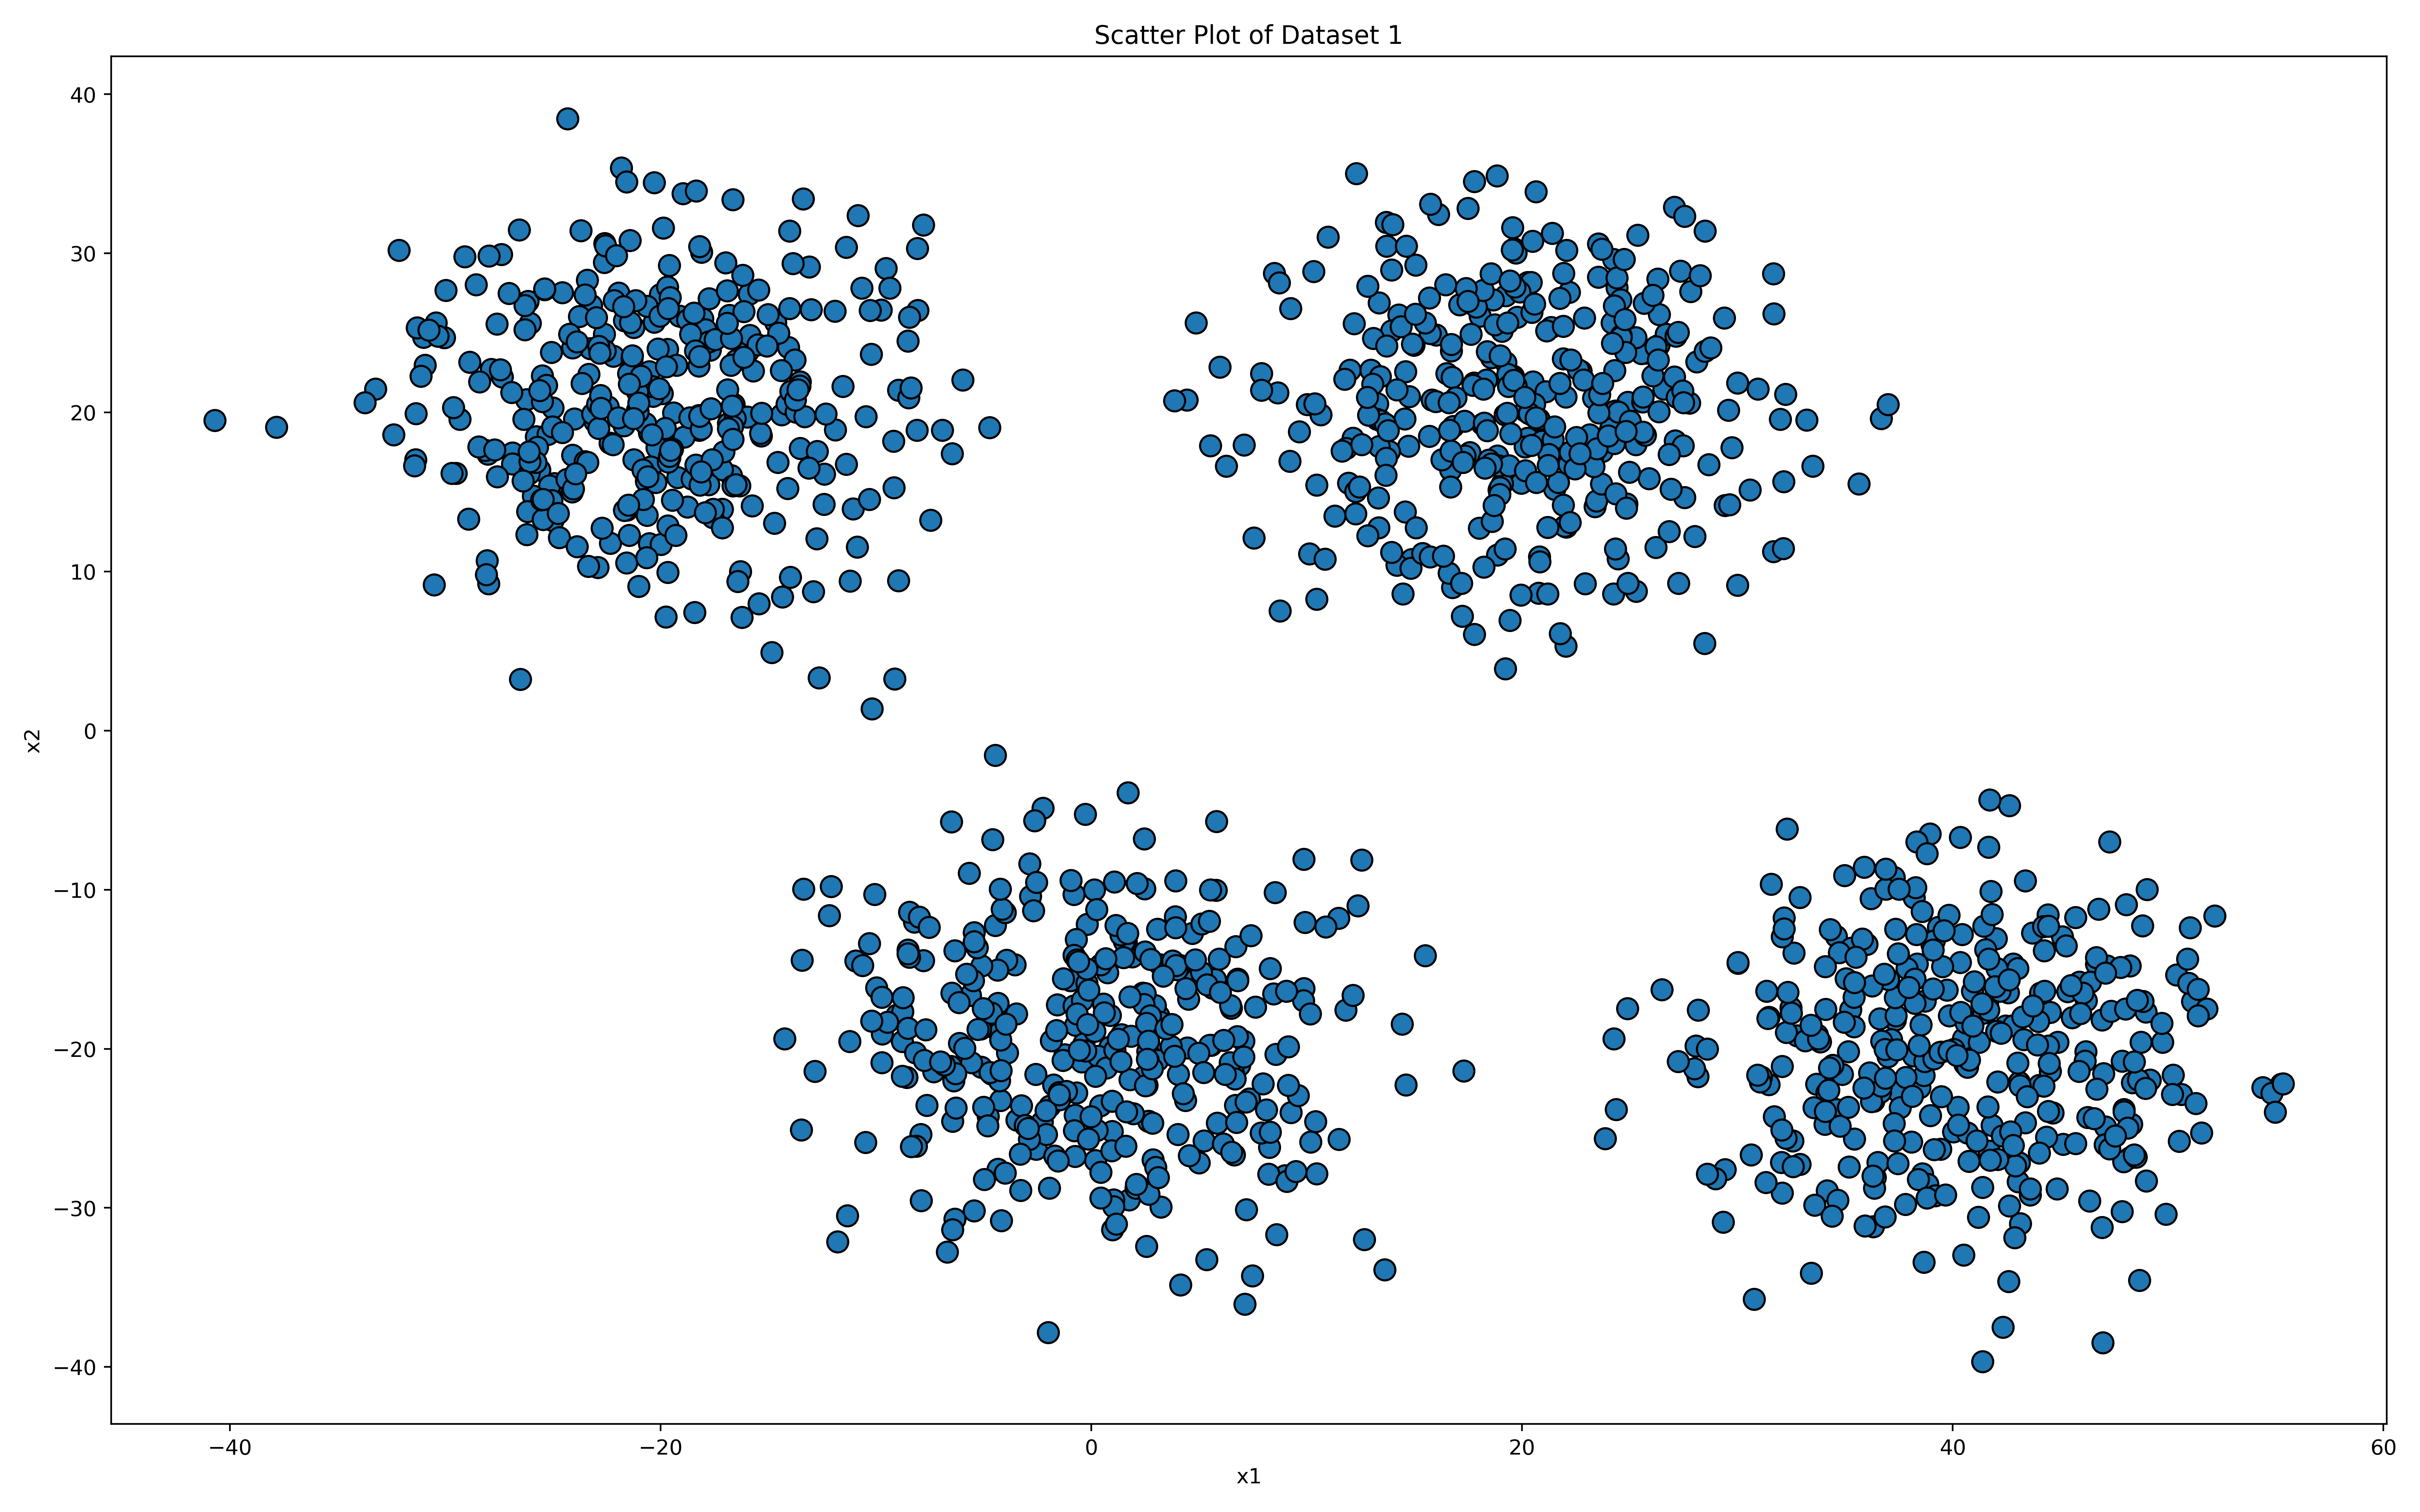
\includegraphics[width=0.8\linewidth]{Images/dataset-1-overview.png}
	\caption{Dataset 1 Overview}
	\label{fig:dataset-1-overview}
\end{figure}

\vspace{10mm}

\subsection*{Dataset 2}

The points in Dataset 2 are distributed in four clusters. The clusters are less well-separated compared to Dataset 1. The points in each cluster are more spread out, and the boundary between clusters is not as clear.

\vspace{10mm}

\begin{figure}[H]
	\centering
	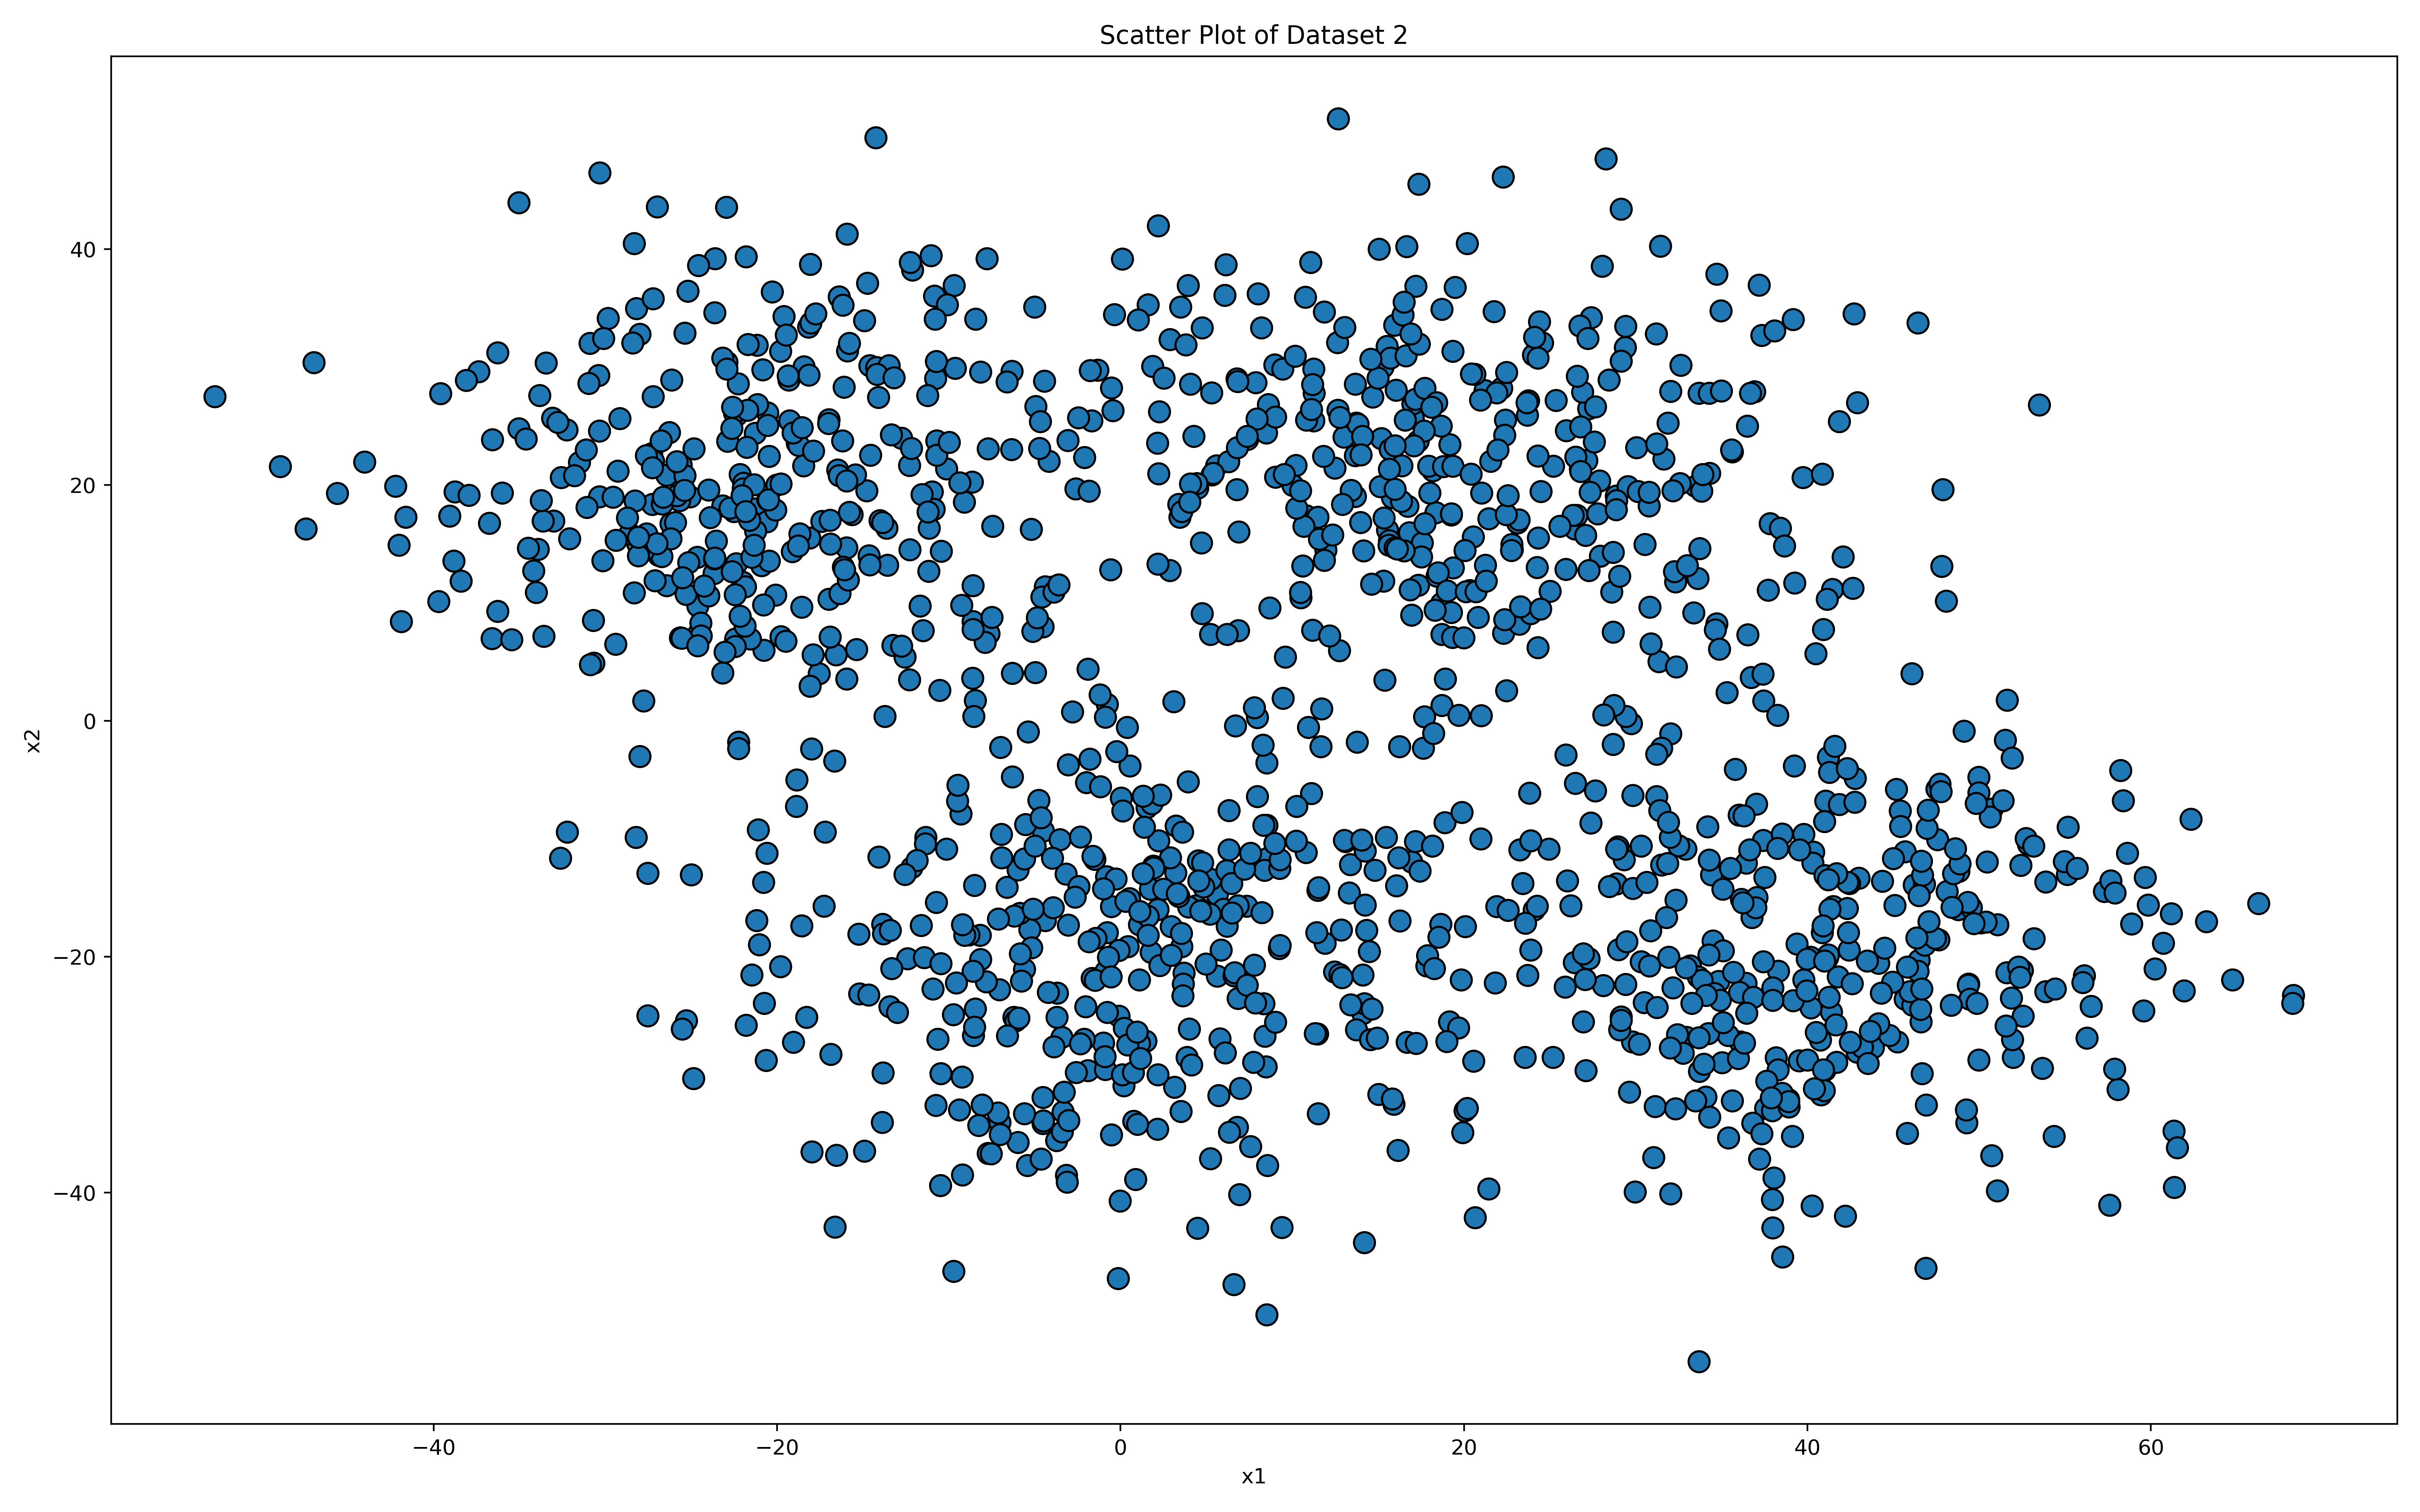
\includegraphics[width=0.8\linewidth]{Images/dataset-2-overview.png}
	\caption{Dataset 2 Overview}
	\label{fig:dataset-2-overview}
\end{figure}

\subsection*{Dataset 3}

The points in Dataset 3 are heavily overlapped and do not form distinct clusters. The points are scattered across the plot without any clear separation. It is challenging to identify clusters based on visual inspection alone.

\begin{figure}[H]
	\centering
	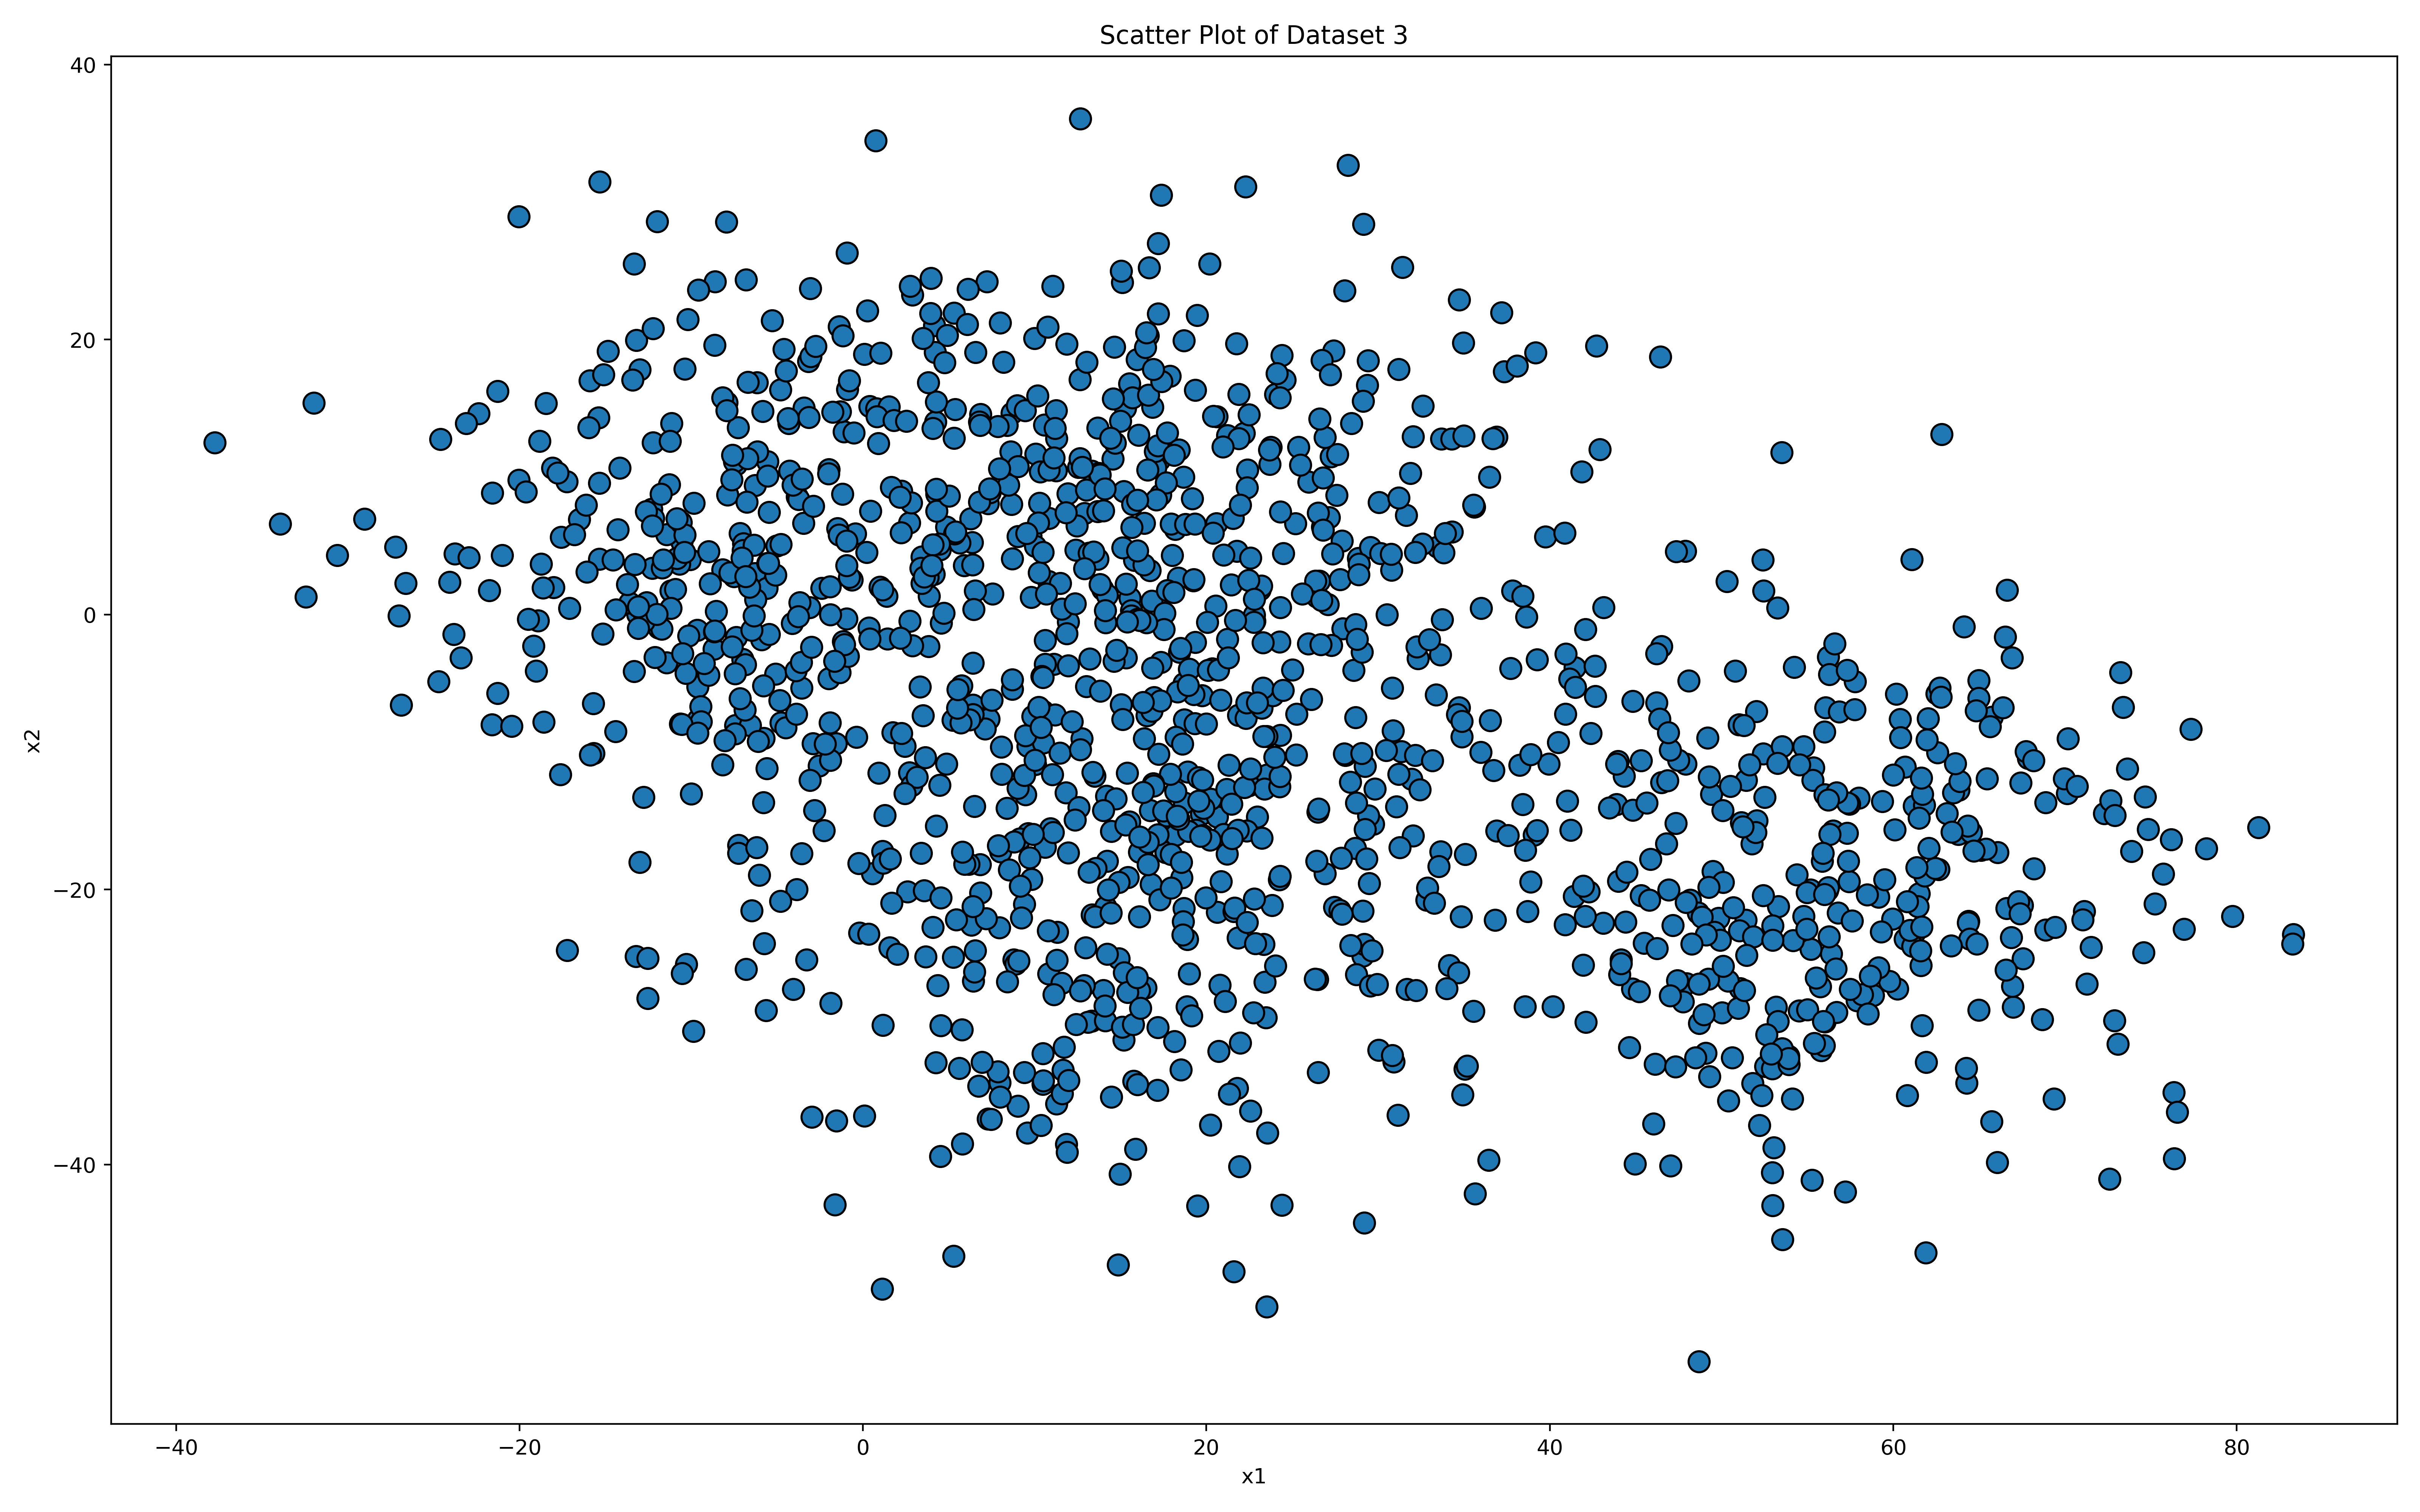
\includegraphics[width=0.8\linewidth]{Images/dataset-3-overview.png}
	\caption{Dataset 3 Overview}
	\label{fig:dataset-3-overview}
\end{figure}

\clearpage

Here is the code used to generate the plots:

\begin{lstlisting}[language=Python, caption=Code to Generate Dataset Plots]
import pandas as pd
import numpy as np
import matplotlib.pyplot as plt
from matplotlib.colors import ListedColormap
from sklearn.model_selection import train_test_split
from sklearn.preprocessing import StandardScaler
from sklearn.cluster import KMeans, AgglomerativeClustering, DBSCAN
from sklearn.metrics import silhouette_score, calinski_harabasz_score, davies_bouldin_score, adjusted_rand_score, confusion_matrix
import os

data_v0 = pd.read_csv('clusters-5-v0.csv')
data_v1 = pd.read_csv('clusters-5-v1.csv')
data_v2 = pd.read_csv('clusters-5-v2.csv')

if not os.path.exists('Images'):
    os.makedirs('Images')

if not os.path.exists('Metrics'):
    os.makedirs('Metrics')

dataset = {
    'Clusters-5-v0': pd.read_csv('clusters-5-v0.csv'),
    'Clusters-5-v1': pd.read_csv('clusters-5-v1.csv'),
    'Clusters-5-v2': pd.read_csv('clusters-5-v2.csv')
}

scalers = {name: StandardScaler().fit_transform(data[['x1', 'x2']]) for name, data in dataset.items()}

datasets = [(data_v0, "Dataset 1"), (data_v1, "Dataset 2"), (data_v2, "Dataset 3")]

for i, (data, label) in enumerate(datasets):
    plt.figure(figsize=(16, 10))
    
    plt.scatter(data['x1'], data['x2'], s=100, edgecolors='black')
    plt.title(f'Scatter Plot of {label}')
    plt.xlabel('x1')
    plt.ylabel('x2')
    
    plt.tight_layout()
    plt.savefig(f'Images/dataset-{i+1}-overview.png', dpi=400)
    plt.show()
\end{lstlisting}

\begin{remark*}
	We use \texttt{os} to create directories for saving images and metrics. We then load the datasets and create a dictionary of datasets. We use the \texttt{StandardScaler} to standardize the data. We iterate over each dataset to create scatter plots of the data points.
\end{remark*}

\clearpage